\documentclass[french]{beamer}
\usetheme{default}

\usepackage[T1]{fontenc}
\usepackage[utf8]{inputenc}
\usepackage{lmodern}
\usepackage{geometry}
\usepackage{babel}
\usepackage{graphicx}
\graphicspath{ {./images/} }

\usepackage{listings}

\usepackage{standalone}

\usepackage{tikz}
\usetikzlibrary{calc,trees,positioning,arrows,chains,shapes.geometric,%
	decorations.pathreplacing,decorations.pathmorphing,shapes,%
	matrix,shapes.symbols,fit,arrows.meta,backgrounds}


\lstset{ %
	texcl=true,
	escapeinside={//}{\^^M},
}

\definecolor{redbackground}{HTML}{ffd4d4}
\definecolor{darkred}{HTML}{b3590b}
\definecolor{blued}{HTML}{384da1}

\title{Étude de quelques algorithmes de joueurs artificiels participants à des jeux de stratégie en temps réel}
\author{Dimitri \bsc{Cocheril-Crèvecœur} \\ 13960}
\begin{document}
\begin{frame}[plain]
    \maketitle
\end{frame}
\begin{frame}{Plan}
	\begin{enumerate}
		\item Présentation du problème
		\item Moteur
		\item Stratégies testées
	\end{enumerate}
\end{frame}
\begin{frame}{StarCraft}
	\begin{figure}
		\centering
		\begin{minipage}{0.5\textwidth}
			Jeu de stratégie en temps réel:
			\begin{itemize}
				\item Jeux simultané
				\item Deux joueurs s'affrontent pour le contrôle d'une carte
				\item Gestion de ressources : minage, création d'unitées, de bases (stratégie)
				\item Combat entre unitées (tactique)
			\end{itemize}
		\end{minipage}\hfill
		\begin{minipage}{0.5\textwidth}
			\centering
			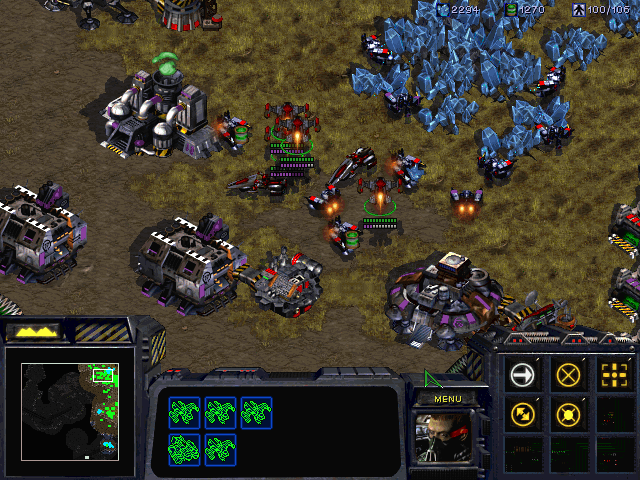
\includegraphics[width=0.99\textwidth]{screen_starcraft.png}
		\end{minipage}
	\end{figure}
\end{frame}
\begin{frame}{Modèles existants}
	\begin{itemize}
		\item IA de Google : \textit{AlphaStar} 
			\\Apprentissage supervisé puis par renforcement
		\item Robots ("bots") :
	\end{itemize}
	\centering
	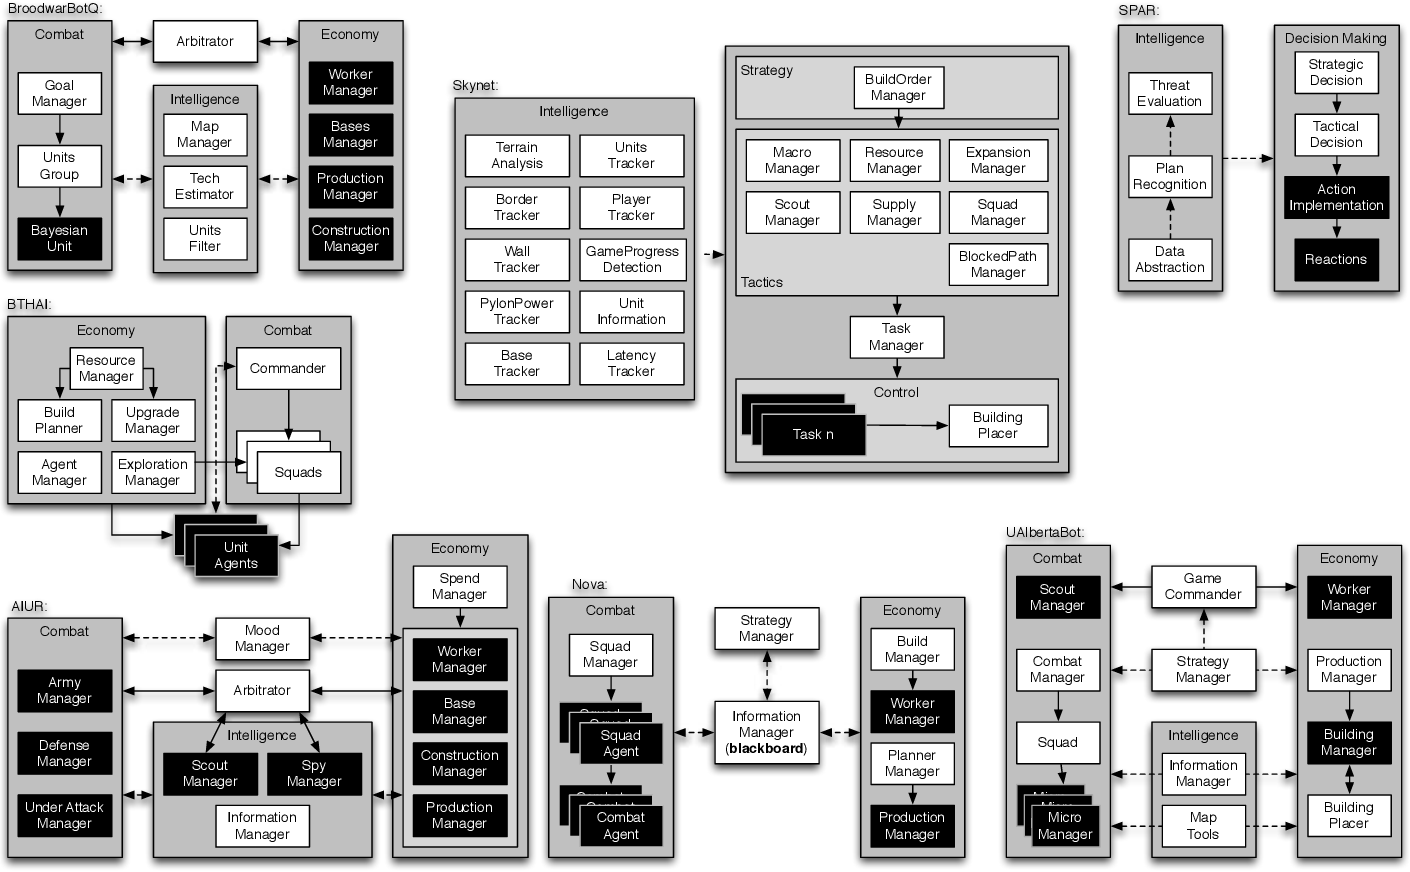
\includegraphics[width=0.7\textwidth]{architectures.png} 
\end{frame}
\begin{frame}{StarCraft}
\begin{figure}
	\centering
	\begin{minipage}{0.45\textwidth}
		On se concentre ici sur la partie "combat" :

		Deux joueurs disposent d'unitées pouvant bouger et attaquer celles adverses

		Chaque joueur doit tuer toute les unitées ennemies
	\end{minipage}\hfill
	\begin{minipage}{0.5\textwidth}
		\centering
		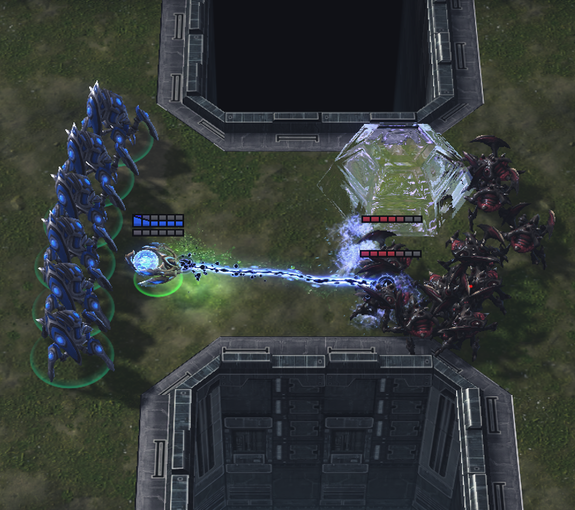
\includegraphics[width=0.99\textwidth]{screen_starcraft_combat.png}
	\end{minipage}
\end{figure}
\end{frame}
\begin{frame}{Problème}
	\begin{enumerate}
		\item Facteur de branchement entre $10^{50}$ et $10^{200}$
		\item Durée typique d'une partie : $25$ minutes donc $25\times60\times24=36000$ états
	\end{enumerate}
\end{frame}
\begin{frame}{Développement moteur du jeu}
	\begin{figure}
		\centering
		\begin{minipage}{0.49\textwidth}
			\centering
			\includestandalone[width=\linewidth]{images/tikz_moteur}
		\end{minipage}\hfill
		\begin{minipage}{0.49\textwidth}
			\centering
			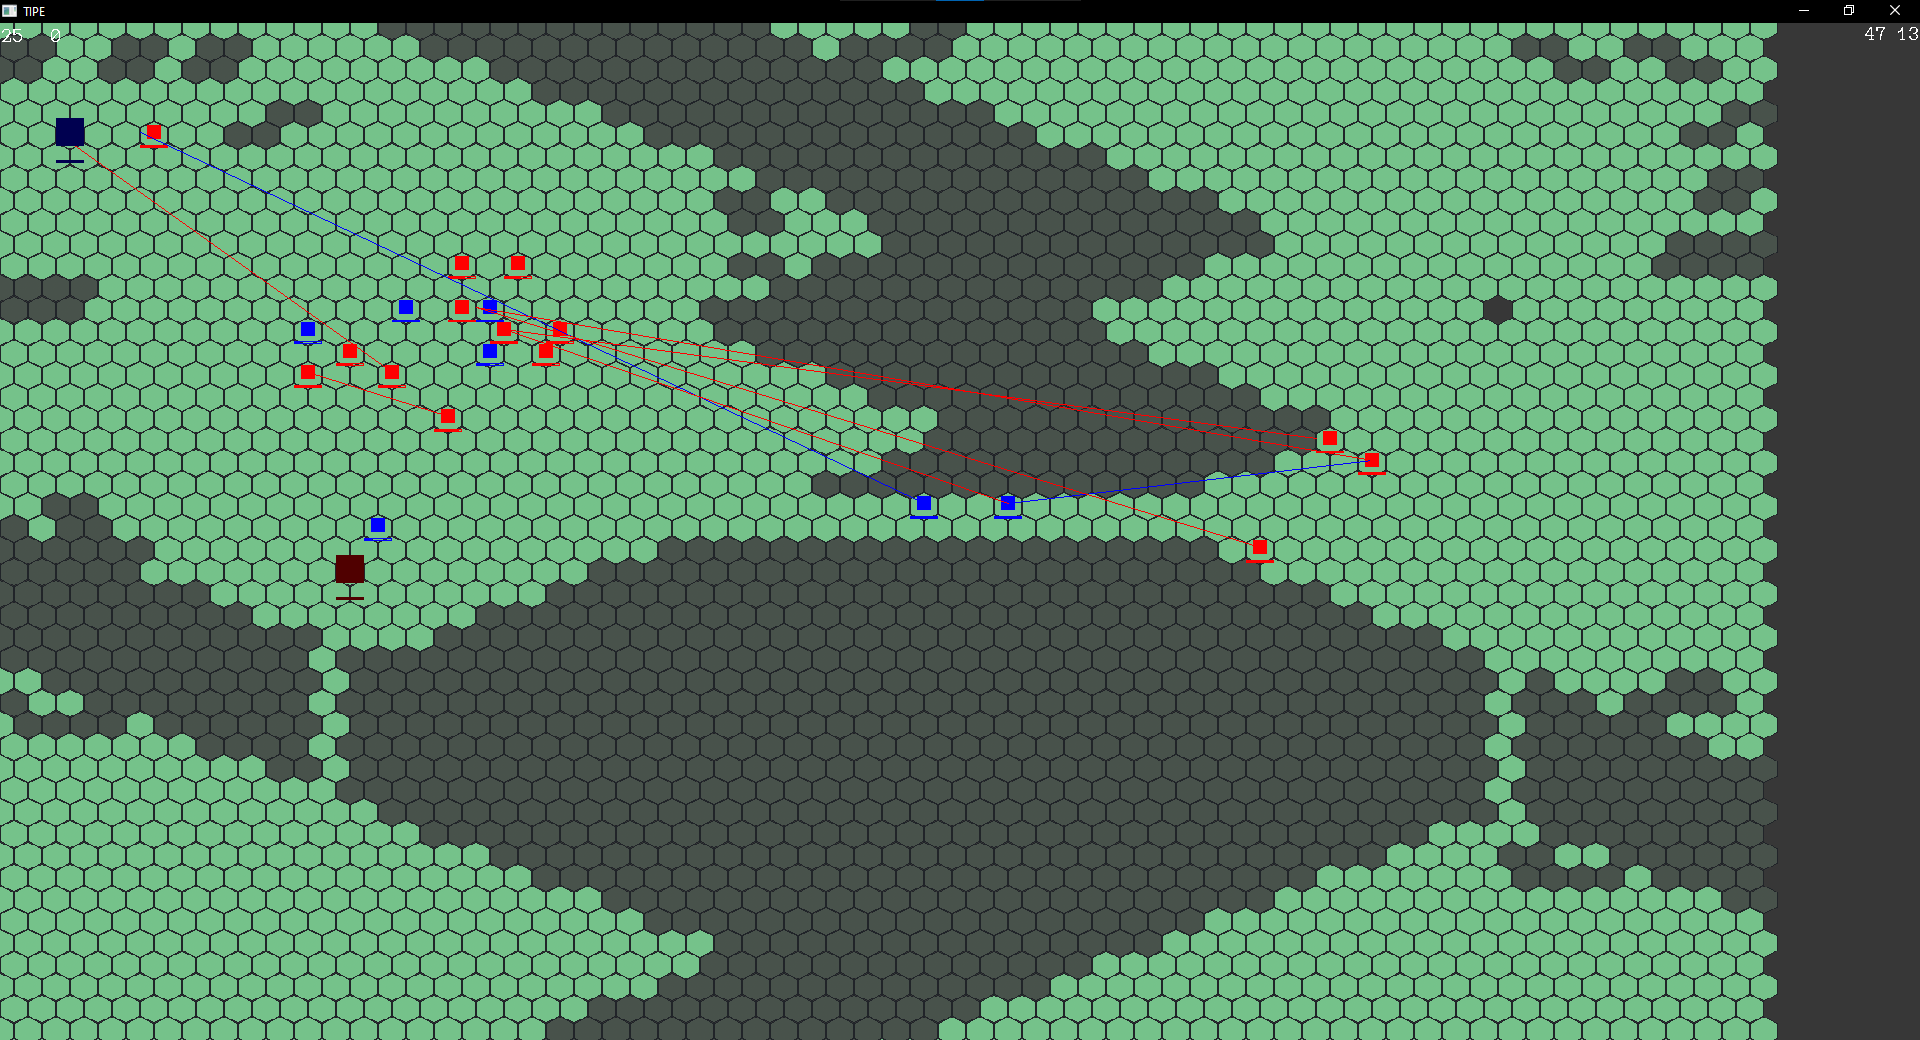
\includegraphics[width=0.95\textwidth]{screen_carte_pleine.png}
		\end{minipage}
	\end{figure}
\end{frame}
\begin{frame}[fragile]
	\small
	\begin{lstlisting}[language=C++,basicstyle=\ttfamily,keywordstyle=\color{red}]
void game_class::play() const
{
    for (const auto p : players_)
    /*Pour chaque joueur...*/
    {
        p->moves_get(this, state_);
        /*..on choisit les actions..*/
    }
    state_->moves_make(map_);
    /*..et on effectue les actions.*/
}
	\end{lstlisting}
\end{frame}
\begin{frame}[fragile]
\small
\begin{lstlisting}[language=C++,basicstyle=\ttfamily,keywordstyle=\color{red}]
	void game_class::play() const
	{
		for (const auto p : players_)
		/*Pour chaque joueur...*/
		{
			p->moves_get(this, state_);
			/*..on choisit les actions..*/
		}
		state_->moves_make(map_);
		/*..et on effectue les actions.*/
	}

\end{lstlisting}
\end{frame}
\begin{frame}{Problème de la recherche de chemin}
	\begin{itemize}
		\item Optimisation compliquée :
		
		On utilise un A* pondérée à 5 (trouvé de manière expérimentale)
		
		\item Parrallélisation du programme
		
		On alloue les espaces dynamiquements au lieu d'utiliser le tas pour éviter la conccurence
	\end{itemize}
Parrallélisation :
\end{frame}
\begin{frame}{Joueur aléatoire}
	Joueur témoin : choisis une action aléatoire, et l'effectue avant d'en choisir une autre aléatoirement
	\vspace*{1em}
	
	On effectue 10000 combats sur une carte vide entre deux joueurs aléatoires avec 50 unités chacun:
	\vspace*{1em}
	
	Victoires de joueur 0 : 4689
	
	Victoires de joueur 1 : 5306
	
	Égalités : 5
\end{frame}
\begin{frame}{Stratégie naïve : attaque par puissance}
	Toutes nos unités attaquent l'unitée ennemie avec la plus grande puissance
	
	Résultats contre joueur aléatoire avec 50 unités:
	
	100\% de victoire pour joueur aléatoire
\end{frame}
\begin{frame}{Utilisation MCTS}
\begin{center}
\scriptsize
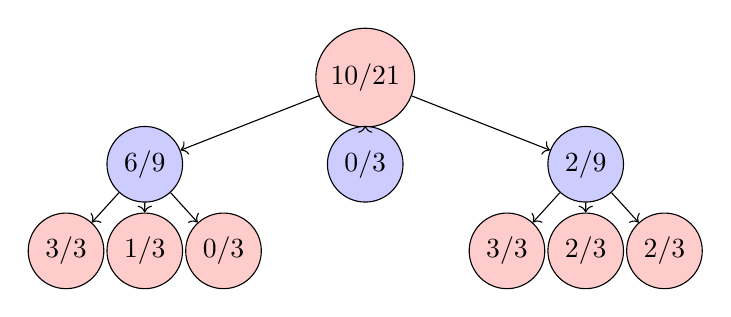
\begin{tikzpicture}[->,
	level distance=11mm,
	level 1/.style={sibling distance=28mm},
	level 2/.style={sibling distance=10mm},]
	\node [circle,draw,fill=red!20] (z){$10/21$}
		child {
		node [circle,draw,fill=blue!20] (a) {$6/9$}
			child {node [circle,draw,fill=red!20]{$3/3$}}
			child {node [circle,draw,fill=red!20]{$1/3$}}
			child {node [circle,draw,fill=red!20]{$0/3$}}
		}
		child {
		node [circle,draw,fill=blue!20] (a) {$0/3$}
		}
		child {
		node [circle,draw,fill=blue!20] (a) {$2/9$}
		child {node [circle,draw,fill=red!20]{$3/3$}}
		child {node [circle,draw,fill=red!20]{$2/3$}}
		child {node [circle,draw,fill=red!20]{$2/3$}}
		}
	;
\end{tikzpicture}
\end{center}
\end{frame}
\begin{frame}{Utilisation MCTS}
	Utilisation de UCT pour la selection : $\frac wn+c\sqrt{\frac{\ln N}n}$
	
	\begin{center}
	Selection et expansion
	\end{center}
\begin{center}
\scriptsize
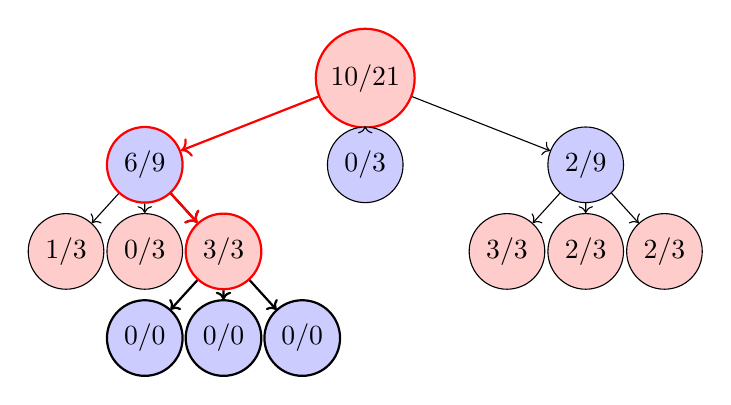
\begin{tikzpicture}[->,
	level distance=11mm,
	level 1/.style={sibling distance=28mm},
	level 2/.style={sibling distance=10mm},
	level 3/.style={sibling distance=10mm},
	level 4/.style={sibling distance=10mm},]
	\node [circle,draw=red,fill=red!20,thick] (z){$10/21$}
		child {
			node [circle,draw=red,fill=blue!20,thick] (a) {$6/9$}
			child {node [circle,draw,fill=red!20]{$1/3$}}
			child {node [circle,draw,fill=red!20]{$0/3$}}
			child {
				node [circle,draw=red,fill=red!20,thick](b){$3/3$} 
				child {
					node [circle,draw,fill=blue!20,thick](c){$0/0$}
				}
				child {
					node [circle,draw,fill=blue!20,thick](c){$0/0$}
				}
				child {
					node [circle,draw,fill=blue!20,thick](c){$0/0$}
				}edge from parent[thick]
			}
			edge from parent[draw=none]
		}
		child {
			node [circle,draw,fill=blue!20] {$0/3$}
		}
		child {
			node [circle,draw,fill=blue!20] {$2/9$}
			child {node [circle,draw,fill=red!20]{$3/3$}}
			child {node [circle,draw,fill=red!20]{$2/3$}}
			child {node [circle,draw,fill=red!20]{$2/3$}}
		}
	;
	\draw[thick,red](z)->(a);
	\draw[thick,red](a)->(b);
\end{tikzpicture}
\end{center}
\end{frame}
\begin{frame}{Utilisation MCTS}
	\begin{center}
		
	Simulation
	\end{center}
\begin{center}
\scriptsize
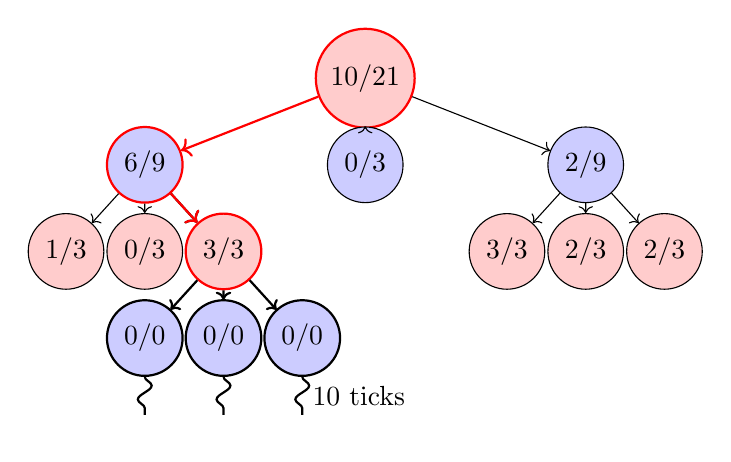
\begin{tikzpicture}[->,
	level distance=11mm,
	level 1/.style={sibling distance=28mm},
	level 2/.style={sibling distance=10mm},
	level 3/.style={sibling distance=10mm},
	level 4/.style={sibling distance=10mm},]


	\node [circle,draw=red,fill=red!20,thick] (z){$10/21$}
		child {
			node [circle,draw=red,fill=blue!20,thick] (a) {$6/9$}
			child {node [circle,draw,fill=red!20]{$1/3$}}
			child {node [circle,draw,fill=red!20]{$0/3$}}
			child {
				node [circle,draw=red,fill=red!20,thick](b){$3/3$} 
				child {
					node [circle,draw,fill=blue!20,thick](e1){$0/0$}
					child {
						node [draw=none](f1){} edge from parent[draw=none]
					} 
				}
				child {
					node [circle,draw,fill=blue!20,thick](e2){$0/0$}
					child {
						node [draw=none](f2){} edge from parent[draw=none]
					} 
				}
				child {
					node [circle,draw,fill=blue!20,thick](e3){$0/0$}
					child {
						node [draw=none](f3){} edge from parent[draw=none]
					} 
				}edge from parent[thick]
			}
			edge from parent[draw=none]
		}
		child {
			node [circle,draw,fill=blue!20] {$0/3$}
		}
		child {
			node [circle,draw,fill=blue!20] {$2/9$}
			child {node [circle,draw,fill=red!20]{$3/3$}}
			child {node [circle,draw,fill=red!20]{$2/3$}}
			child {node [circle,draw,fill=red!20]{$2/3$}}
		}
	;
	\draw[thick,red](z)->(a);
	\draw[thick,red](a)->(b);
	\draw[decoration=snake,decorate, thick,-](e1)--(f1);
	\draw[decoration=snake,decorate, thick,-](e2)--(f2);
	\draw[decoration=snake,decorate, thick,-](e3)--(f3)node [midway, right]{10 ticks};
\end{tikzpicture}
\end{center}
\end{frame}
\begin{frame}{Rassemblement des unitées : DBSCAN}
	\begin{minipage}{0.5\textwidth}
		\centering
		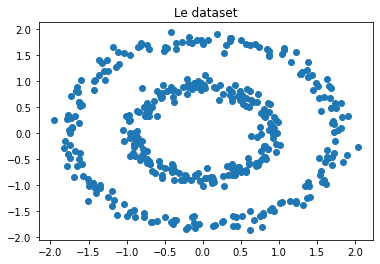
\includegraphics[width=0.99\textwidth]{circles.png}
		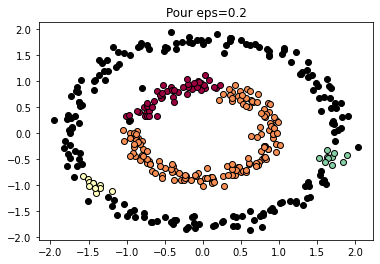
\includegraphics[width=0.99\textwidth]{petit_eps.png}
	\end{minipage}\hfill
	\begin{minipage}{0.5\textwidth}
		\centering
		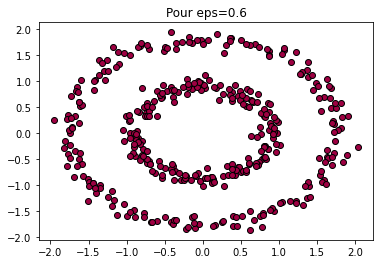
\includegraphics[width=0.99\textwidth]{grand_eps.png}
		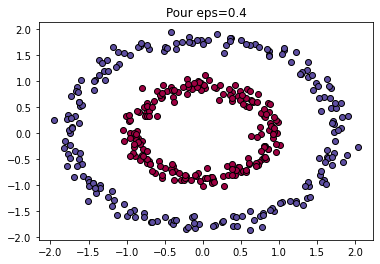
\includegraphics[width=0.99\textwidth]{dbscan.png}
	\end{minipage}
\end{frame}
\begin{frame}{Rassemblement des unitées : DBSCAN}
	Deux paramètres : $\varepsilon$ et $MinPts$

	Ici avec $MinPts = 3$ :

\vspace*{1em}

\begin{center}
\begin{tikzpicture}[scale=0.8,baseline = (current bounding box.center)]
	
    \draw[red, fill=red](0,0) circle (2 pt);

    \draw[fill=black](0.3,0.2) circle (1.5pt);
    \draw[fill=black](-0.2,0.4) circle (1.5pt);
    \draw[fill=black](-0.1,0.6) circle (1.5pt);
    \draw[fill=black](0.2,-0.3) circle (1.5pt);
    \draw[fill=black](-0.2,-0.5) circle (1.5pt);

    \draw[fill=black](-1,-1) circle (1.5pt);

    \draw[fill=black](1.4,0.6) circle (1.5pt);
    \draw[fill=black](1.7,0.8) circle (1.5pt);
    \draw[fill=black](1.6,1) circle (1.5pt);
    \draw[fill=black](1.9,0.6) circle (1.5pt);
    \draw[fill=black](2,0.9) circle (1.5pt);
    \draw[fill=black](1.1,1.3) circle (1.5pt);

\end{tikzpicture}
$\longrightarrow$
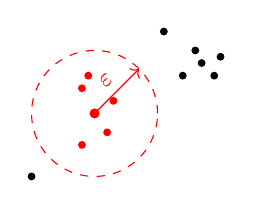
\begin{tikzpicture}[scale=0.8,baseline = (current bounding box.center)]
	
    \draw[red, fill=red](0,0) circle (2 pt);

    \draw[fill=red,red](0.3,0.2) circle (1.5pt);
    \draw[fill=red,red](-0.2,0.4) circle (1.5pt);
    \draw[fill=red,red](-0.1,0.6) circle (1.5pt);
    \draw[fill=red,red](0.2,-0.3) circle (1.5pt);
    \draw[fill=red,red](-0.2,-0.5) circle (1.5pt);

    \draw[fill=black](-1,-1) circle (1.5pt);

    \draw[fill=black](1.4,0.6) circle (1.5pt);
    \draw[fill=black](1.7,0.8) circle (1.5pt);
    \draw[fill=black](1.6,1) circle (1.5pt);
    \draw[fill=black](1.9,0.6) circle (1.5pt);
    \draw[fill=black](2,0.9) circle (1.5pt);
    \draw[fill=black](1.1,1.3) circle (1.5pt);

    \draw[fill=none,red,dashed](0,0) circle (1.0);
    \draw[red,->](0,0) -> (0.707,0.707) node [midway, above, sloped]{\small$\varepsilon$};
\end{tikzpicture}
$\longrightarrow$
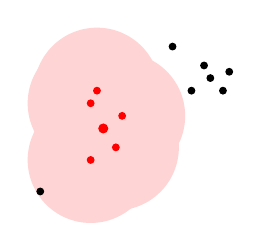
\begin{tikzpicture}[scale=0.8,baseline = (current bounding box.center)]

    \draw[fill=redbackground,draw=none](0.3,0.2) circle (1.0);
    \draw[fill=redbackground,draw=none](-0.2,0.4) circle (1.0);
    \draw[fill=redbackground,draw=none](-0.1,0.6) circle (1.0);
    \draw[fill=redbackground,draw=none](0.2,-0.3) circle (1.0);
    \draw[fill=redbackground,draw=none](-0.2,-0.5) circle (1.0);

    \draw[red, fill=red](0,0) circle (2 pt);

    \draw[fill=red,red](0.3,0.2) circle (1.5pt);
    \draw[fill=red,red](-0.2,0.4) circle (1.5pt);
    \draw[fill=red,red](-0.1,0.6) circle (1.5pt);
    \draw[fill=red,red](0.2,-0.3) circle (1.5pt);
    \draw[fill=red,red](-0.2,-0.5) circle (1.5pt);

    \draw[fill=black](-1,-1) circle (1.5pt);

    \draw[fill=black](1.4,0.6) circle (1.5pt);
    \draw[fill=black](1.7,0.8) circle (1.5pt);
    \draw[fill=black](1.6,1) circle (1.5pt);
    \draw[fill=black](1.9,0.6) circle (1.5pt);
    \draw[fill=black](2,0.9) circle (1.5pt);
    \draw[fill=black](1.1,1.3) circle (1.5pt);
\end{tikzpicture}
\end{center}

\begin{center}
$\longrightarrow$
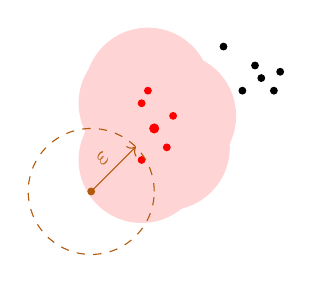
\begin{tikzpicture}[scale=0.8,baseline = (current bounding box.center)]

    \draw[fill=redbackground,draw=none](0.3,0.2) circle (1.0);
    \draw[fill=redbackground,draw=none](-0.2,0.4) circle (1.0);
    \draw[fill=redbackground,draw=none](-0.1,0.6) circle (1.0);
    \draw[fill=redbackground,draw=none](0.2,-0.3) circle (1.0);
    \draw[fill=redbackground,draw=none](-0.2,-0.5) circle (1.0);

    \draw[red, fill=red](0,0) circle (2 pt);

    \draw[fill=red,red](0.3,0.2) circle (1.5pt);
    \draw[fill=red,red](-0.2,0.4) circle (1.5pt);
    \draw[fill=red,red](-0.1,0.6) circle (1.5pt);
    \draw[fill=red,red](0.2,-0.3) circle (1.5pt);
    \draw[fill=red,red](-0.2,-0.5) circle (1.5pt);

    \draw[fill=darkred,darkred](-1,-1) circle (1.5pt);
    \draw[fill=none,darkred,dashed](-1,-1) circle (1.0);
    \draw[darkred,->](-1,-1) -> (-0.293,-0.293) node [midway, above, sloped]{\small$\varepsilon$};

    \draw[fill=black](1.4,0.6) circle (1.5pt);
    \draw[fill=black](1.7,0.8) circle (1.5pt);
    \draw[fill=black](1.6,1) circle (1.5pt);
    \draw[fill=black](1.9,0.6) circle (1.5pt);
    \draw[fill=black](2,0.9) circle (1.5pt);
    \draw[fill=black](1.1,1.3) circle (1.5pt);
\end{tikzpicture}
$\rightarrow$
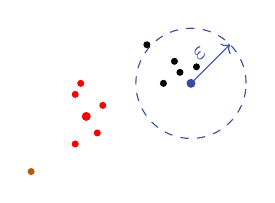
\begin{tikzpicture}[scale=0.7,baseline = (current bounding box.center)]

    \draw[red, fill=red](0,0) circle (2 pt);

    \draw[fill=red,red](0.3,0.2) circle (1.5pt);
    \draw[fill=red,red](-0.2,0.4) circle (1.5pt);
    \draw[fill=red,red](-0.1,0.6) circle (1.5pt);
    \draw[fill=red,red](0.2,-0.3) circle (1.5pt);
    \draw[fill=red,red](-0.2,-0.5) circle (1.5pt);

    \draw[fill=darkred,darkred](-1,-1) circle (1.5pt);

    \draw[fill=black](1.4,0.6) circle (1.5pt);
    \draw[fill=black](1.7,0.8) circle (1.5pt);
    \draw[fill=black](1.6,1) circle (1.5pt);
    \draw[blued, fill](1.9,0.6) circle (2pt);

	\draw[fill=none,blued,dashed](1.9,0.6) circle (1.0);
    \draw[blued,->](1.9,0.6) -> (2.607,1.307) node [midway, above, sloped]{\small$\varepsilon$};

    \draw[fill=black](2,0.9) circle (1.5pt);
    \draw[fill=black](1.1,1.3) circle (1.5pt);

\end{tikzpicture}
$\rightarrow$
\begin{tikzpicture}[scale=0.8,baseline = (current bounding box.center)]
	

    \draw[red, fill=red](0,0) circle (2 pt);

    \draw[red, fill](0.3,0.2) circle (1.5pt);
    \draw[red, fill](-0.2,0.4) circle (1.5pt);
    \draw[red, fill](-0.1,0.6) circle (1.5pt);
    \draw[red, fill](0.2,-0.3) circle (1.5pt);
    \draw[red, fill](-0.2,-0.5) circle (1.5pt);

    \draw[darkred, fill](-1,-1) circle (1.5pt);

    \draw[blued, fill](1.4,0.6) circle (1.5pt);
    \draw[blued, fill](1.7,0.8) circle (1.5pt);
    \draw[blued, fill](1.6,1) circle (1.5pt);
    \draw[blued, fill](1.9,0.6) circle (1.5pt);
    \draw[blued, fill](2,0.9) circle (1.5pt);
    \draw[blued, fill](1.1,1.3) circle (1.5pt);

	\draw[fill=none,blued,dashed](1.1,1.3) circle (1.0);
\end{tikzpicture}
\end{center}

Points {\color{darkred}frontière et }{\color{red} centraux du cluster 1 et }{\color{blued}du cluster 2}
\end{frame}

\begin{frame}{Application du DBSCAN}
	
\end{frame}
\end{document}
